% ****** Start of file aipsamp.tex ******
%
%   This file is part of the AIP files in the AIP distribution for REVTeX 4.
%   Version 4.1 of REVTeX, October 2009
%
%   Copyright (c) 2009 American Institute of Physics.
%
%   See the AIP README file for restrictions and more information.
%
% TeX'ing this file requires that you have AMS-LaTeX 2.0 installed
% as well as the rest of the prerequisites for REVTeX 4.1
%
% It also requires running BibTeX. The commands are as follows:
%
%  1)  latex  aipsamp
%  2)  bibtex aipsamp
%  3)  latex  aipsamp
%  4)  latex  aipsamp
%
% Use this file as a source of example code for your aip document.
% Use the file aiptemplate.tex as a template for your document.
\documentclass[%
 aip,
 jmp,
 amsmath,
 amssymb,
%preprint,%
 reprint,%
%author-year,%
%author-numerical,%
 numerical,
 longbibliography,
]{revtex4-1}

\usepackage{graphicx}% Include figure files
\graphicspath{{images/}}
\usepackage{dcolumn}% Align table columns on decimal point
\usepackage{bm}% bold math
\usepackage{url}
\usepackage{float}
\usepackage{silence}
\usepackage{tabularx}
\usepackage{verbatimbox}
\WarningFilter{revtex4-1}{Repair the float}
%\usepackage[mathlines]{lineno}% Enable numbering of text and display math
%\linenumbers\relax % Commence numbering lines

\begin{document}

%\preprint{AIP/123-QED}

\title[Laboratory 4]{Switches} % Force line breaks with \\

\author{Kevin "Yama" Keyser}
 \email{kk8r8@mail.umck.edu}
\affiliation{ 
	University of Missouri-Kansas City
	%\\This line break forced with \textbackslash\textbackslash
}%

%\date{\today}% It is always \today, today,
             %  but any date may be explicitly specified

\begin{abstract}

Laboratory 4 has us focusing on electromechanical relay switches, and solid-state
switches. This is to see the differences between a physical bounce that is caused
by a restoring force from a spring, and the same type of restoring force that can
be seen from a capacitor. We will also see the limitations of a physical arm used
to trigger a switch, and at what limit does the electromechanical relay switch 
stop being effective.

\end{abstract}

%\keywords{Operational Amplifier}%Use showkeys class option if keyword
                              %display desired
\maketitle

%\begin{quotation}
%The ``lead paragraph'' is encapsulated with the \LaTeX\ 
%\verb+quotation+ environment and is formatted as a single paragraph before the first section heading. 
%(The \verb+quotation+ environment reverts to its usual meaning after the first sectioning command.) 
%Note that numbered references are allowed in the lead paragraph.
%
%The lead paragraph will only be found in an article being prepared for the journal \textit{Chaos}.
%\end{quotation}

\section{Background}

Laboratory 4 didn't require much background knowledge that we didn't already have. This included
the use of an oscilloscope, and following a basic circuit diagram.

\section{Procedure}

The procedures for Laboratory 4 will be attached as a separate sheet of paper to the back
of the laboratory write up.

\section{Presentation of Data}

	\subsection{4-1: Electromechanical Relay Switches}
	
	\begin{figure}[H]
	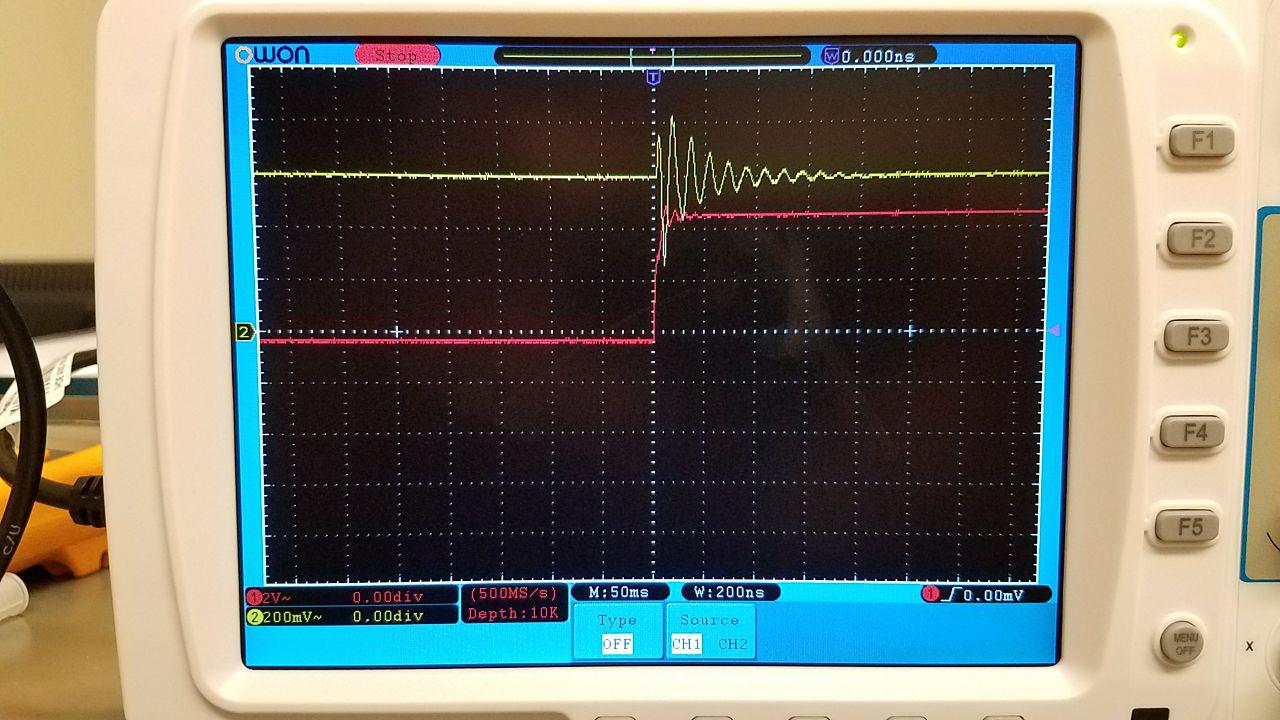
\includegraphics[width=\columnwidth]{41-10Hz.eps}
	\caption{Input and Output of our circuit at 10Hz.\\
	Output is scaled to 200mV increments.}
	\end{figure}	
	
	\begin{figure}[H]
	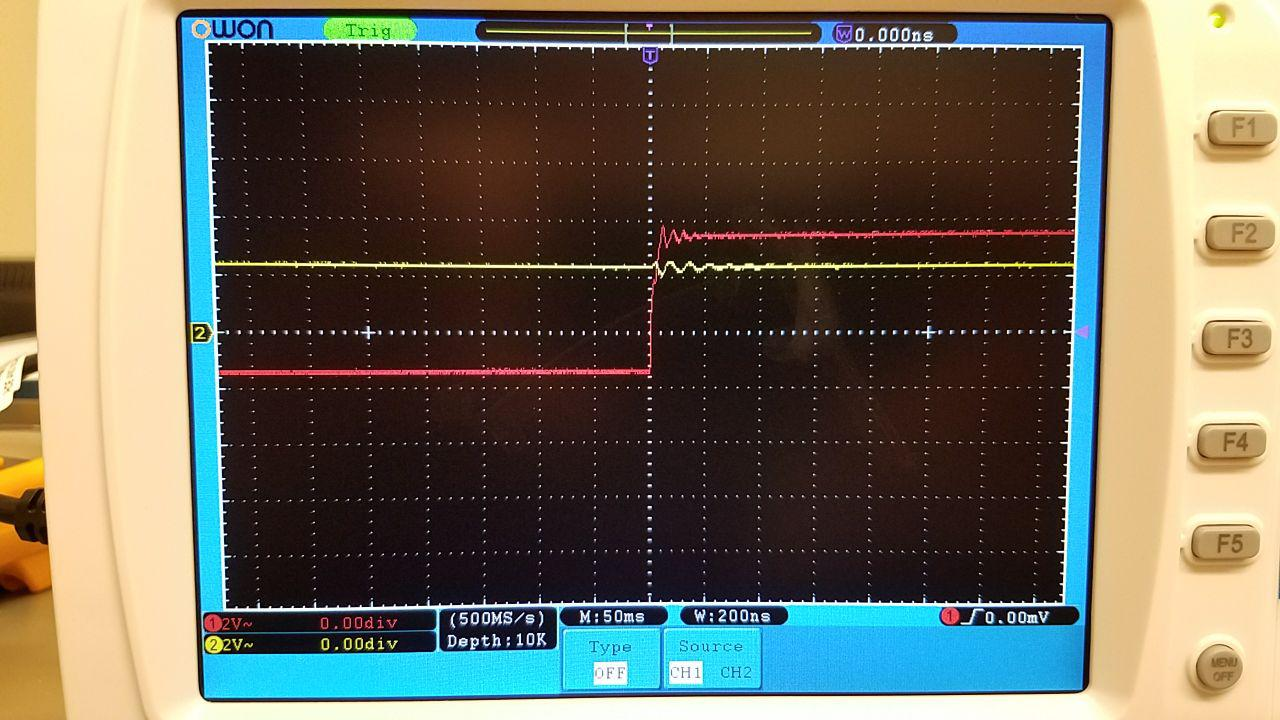
\includegraphics[width=\columnwidth]{41-50Hz.eps}
	\caption{Input and Output of our circuit at 10Hz.}
	\end{figure}
	
	\begin{figure}[H]
	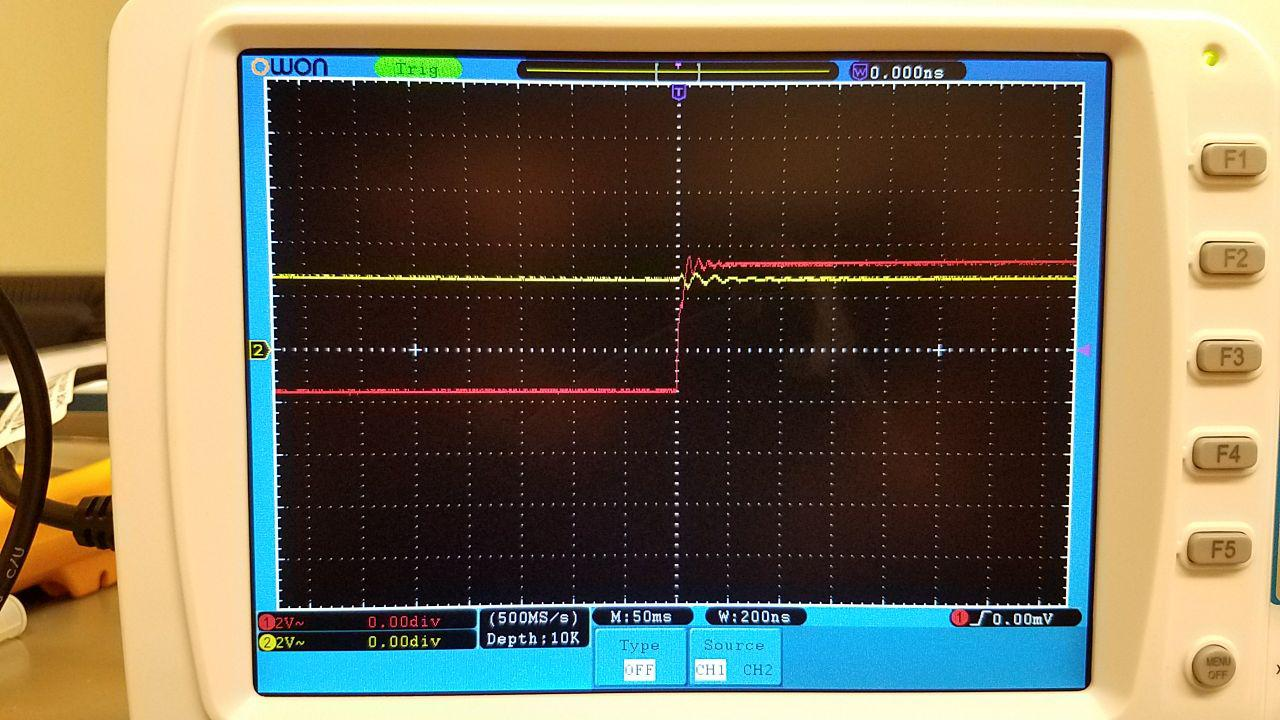
\includegraphics[width=\columnwidth]{41-75Hz.eps}
	\caption{Input and Output of our circuit at 10Hz.}
	\end{figure}
	
	\begin{tabularx}{0.45\textwidth}[t]{| X | X |}
	\hline
	\multicolumn{2}{|c|}{Freq. of Failure (Hz)}\\
	\hline
	Destabalized & 145 \\ \hline
	Complete Failure & 160 \\ \hline
	\end{tabularx}

	\subsection{4-2: Solid-State Switches}
	
	\begin{figure}[H]
	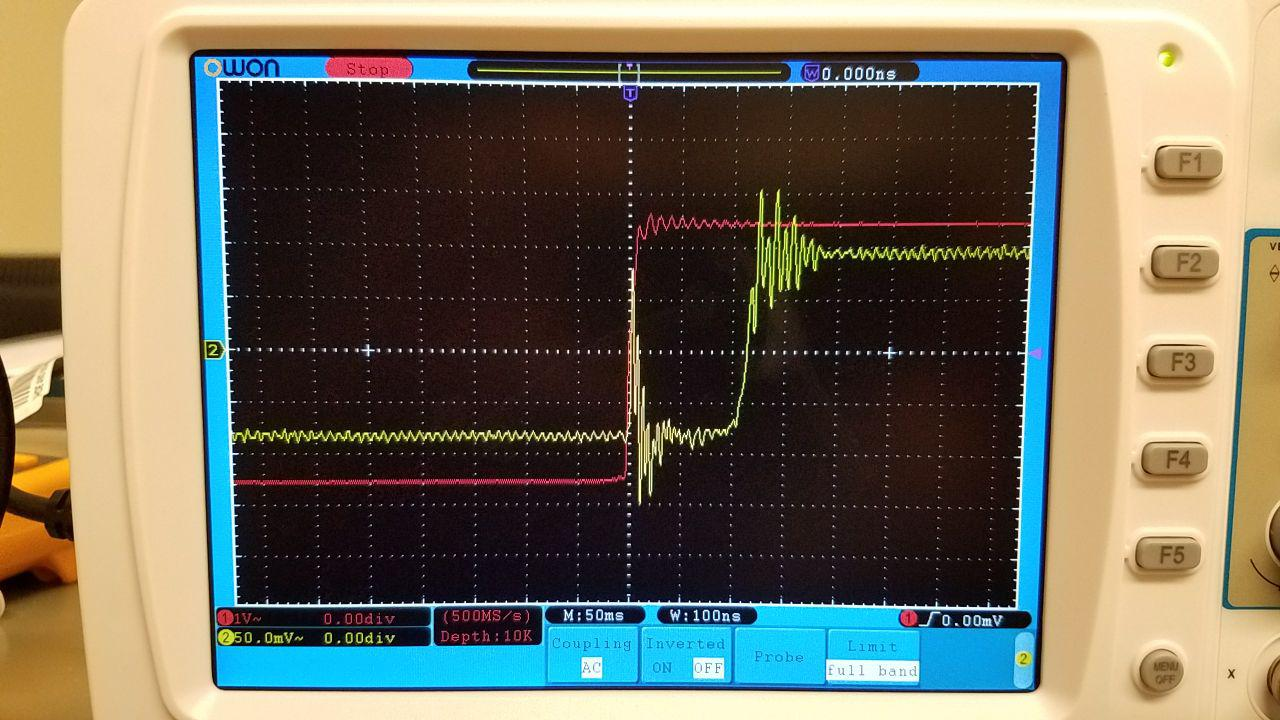
\includegraphics[width=\columnwidth]{42-10kHzStart.eps}
	\caption{Time delay at 10kHz from off to on.}
	\end{figure}	
	
	\begin{figure}[H]
	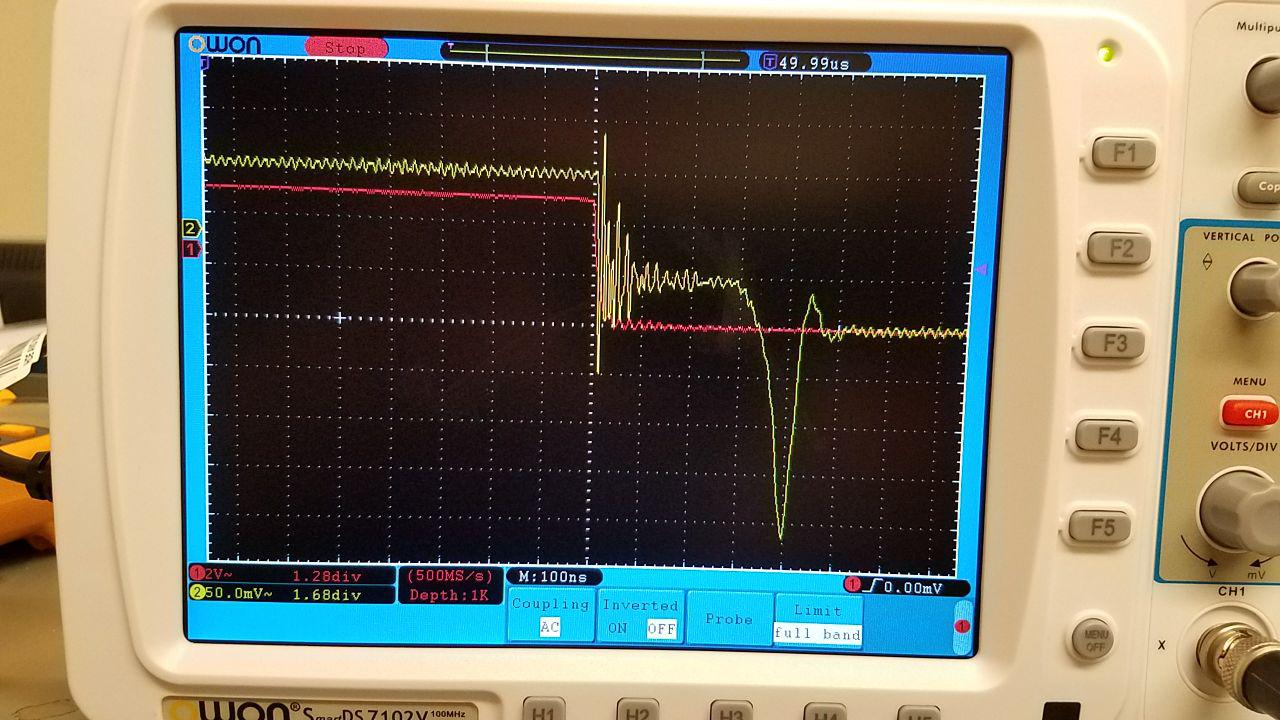
\includegraphics[width=\columnwidth]{42-10kHzEnd.eps}
	\caption{Time delay at 10kHz from on to off.}
	\end{figure}
	
	\begin{figure}[H]
	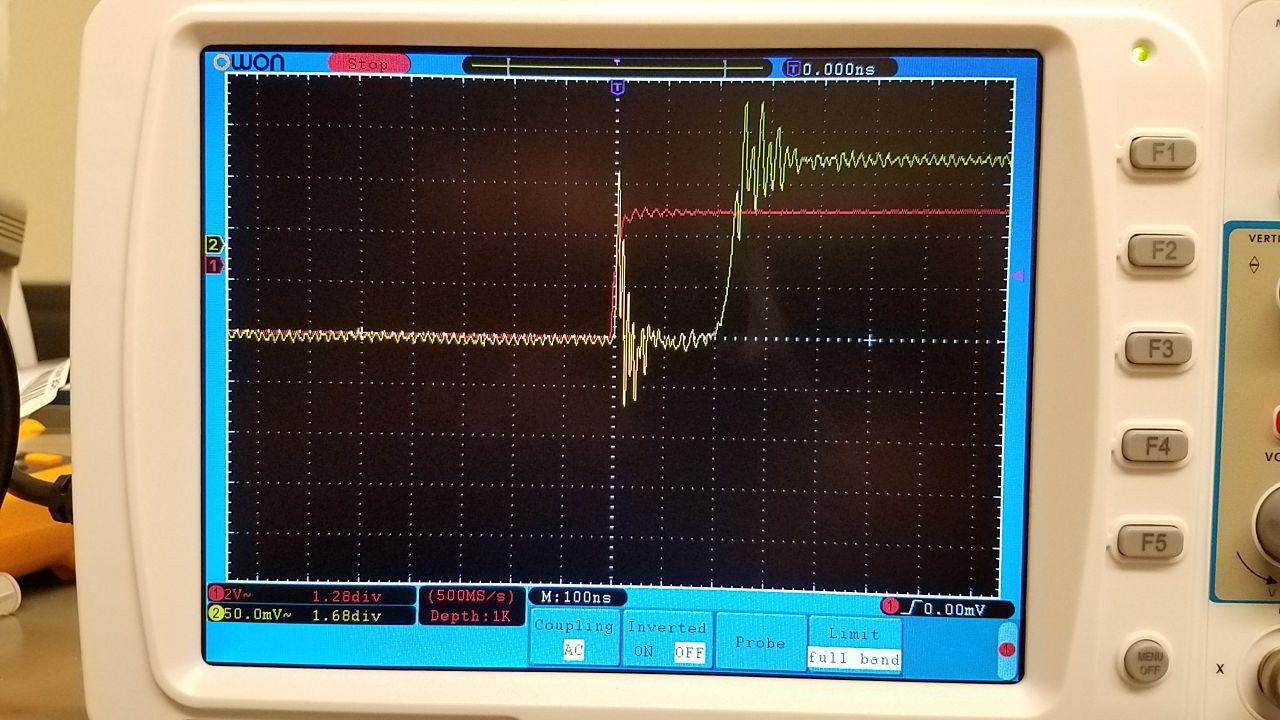
\includegraphics[width=\columnwidth]{42-50kHzStart.eps}
	\caption{Time delay at 50kHz from off to on.}
	\end{figure}	
	
	\begin{figure}[H]
	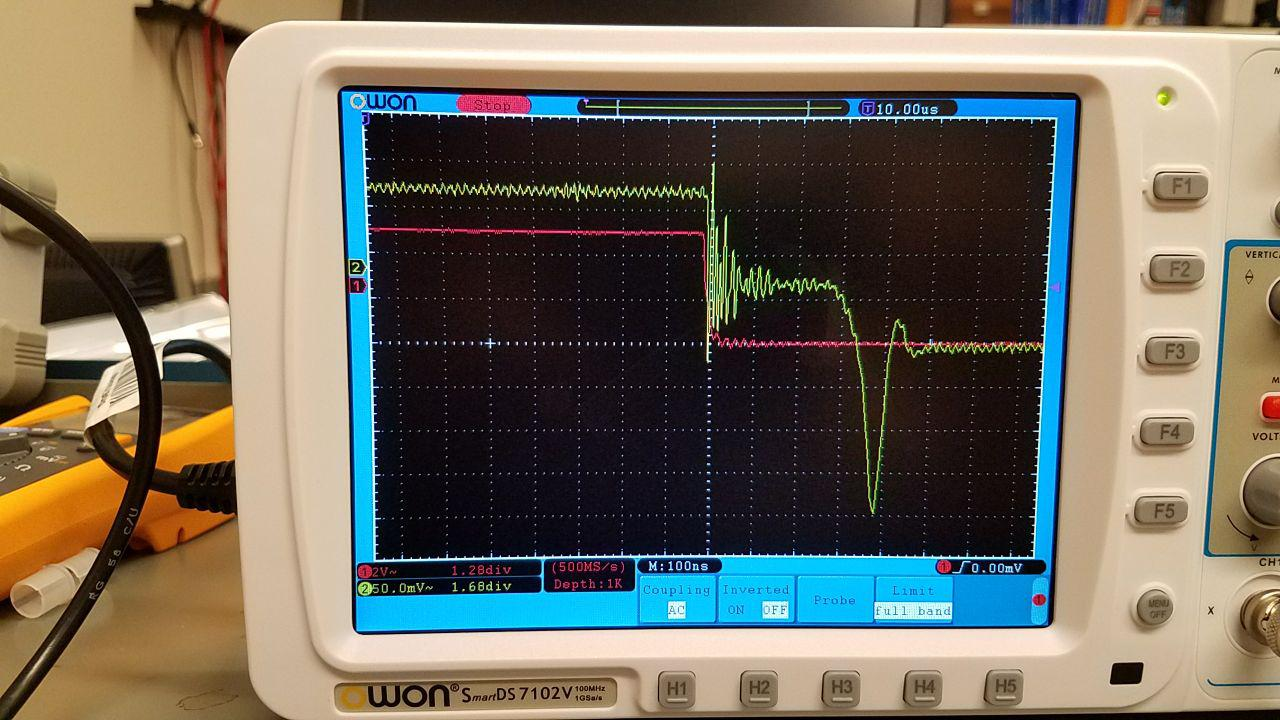
\includegraphics[width=\columnwidth]{42-50kHzEnd.eps}
	\caption{Time delay at 50kHz from on to off.}
	\end{figure}
	
	\begin{figure}[H]
	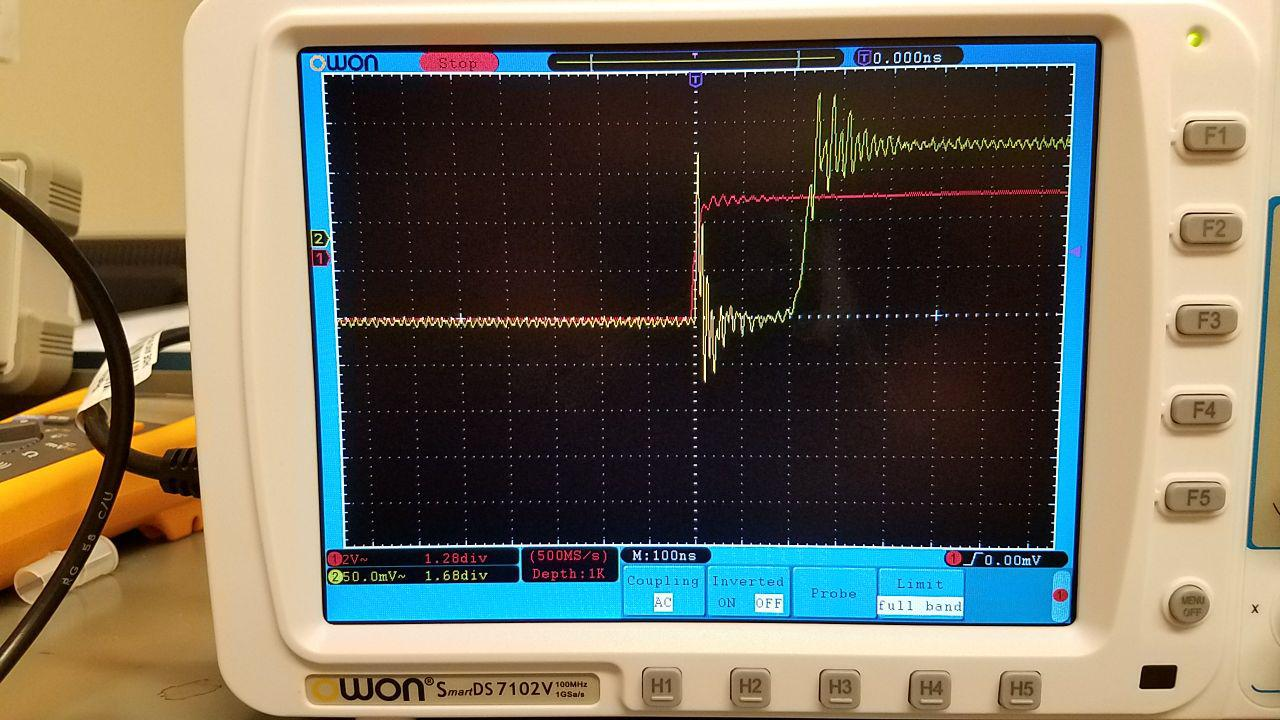
\includegraphics[width=\columnwidth]{42-100kHzStart.eps}
	\caption{Time delay at 100kHz from off to on.}
	\end{figure}	
	
	\begin{figure}[H]
	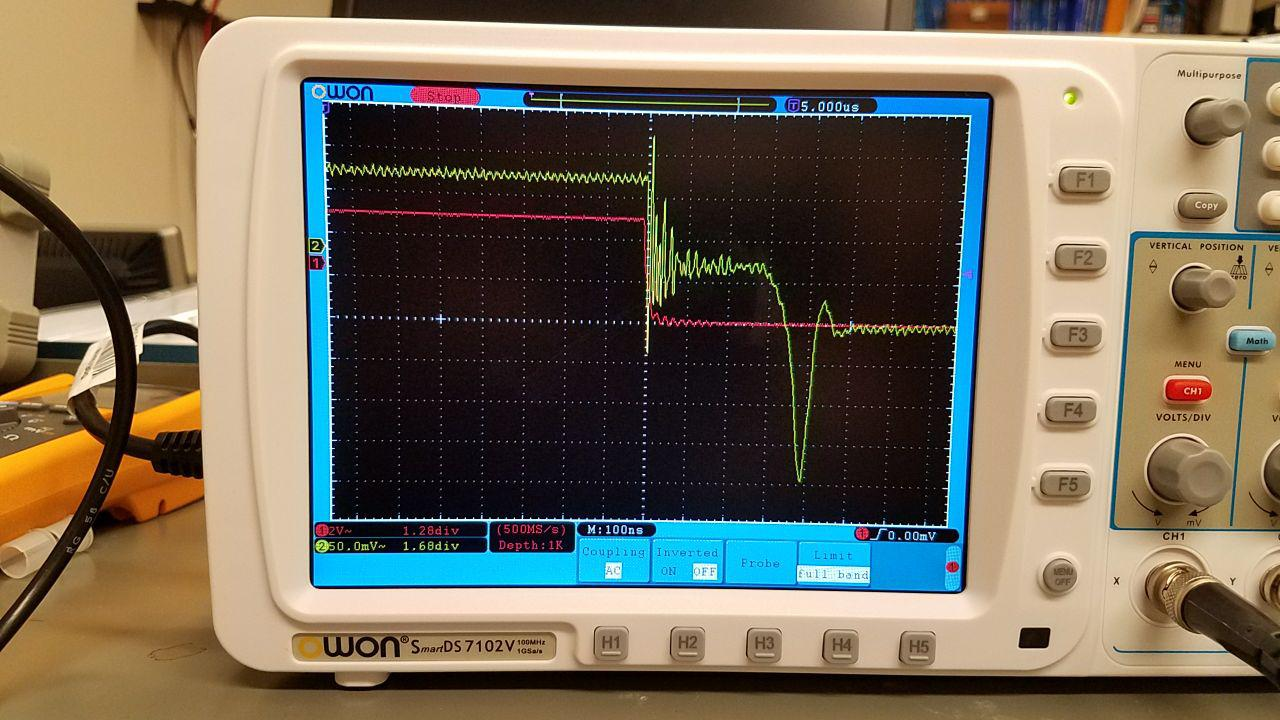
\includegraphics[width=\columnwidth]{42-100kHzEnd.eps}
	\caption{Time delay at 100kHz from on to off.}
	\end{figure}
	
	\begin{tabularx}{0.45\textwidth}[t]{| X | X | X | X |}
	\hline
	\multicolumn{4}{|c|}{Transition Times (s)}\\
	\hline
	\multicolumn{4}{|c|}{10kHz}\\
	\hline	
	\multicolumn{1}{|c|}{td} & \multicolumn{1}{c|}{tr} & \multicolumn{1}{c|}{td'} & \multicolumn{1}{c|}{tf}\\ \hline
	\hline
	71.6$\mu s$ & $<$80$ns$ & 59.0$\mu s$ & 32.6$\mu s$ \\ \hline
	\multicolumn{4}{|c|}{50kHz}\\
	\hline	
	\multicolumn{1}{|c|}{td} & \multicolumn{1}{c|}{tr} & \multicolumn{1}{c|}{td'} & \multicolumn{1}{c|}{tf}\\ \hline
	\hline
	10.32$\mu s$ & $<$40$ns$ & 14.88$\mu s$ & 3.08$\mu s$ \\ \hline
	\multicolumn{4}{|c|}{100kHz}\\
	\hline	
	\multicolumn{1}{|c|}{td} & \multicolumn{1}{c|}{tr} & 
	\multicolumn{1}{c|}{td'} & \multicolumn{1}{c|}{tf}\\ \hline
	\hline
	5.32$\mu s$ & $<$20$ns$ & 9.92$\mu s$ & 120$ns$ \\ \hline
	\end{tabularx}
	
	\subsection{4-3: Transistor Switches}
	
	\begin{figure}[H]
	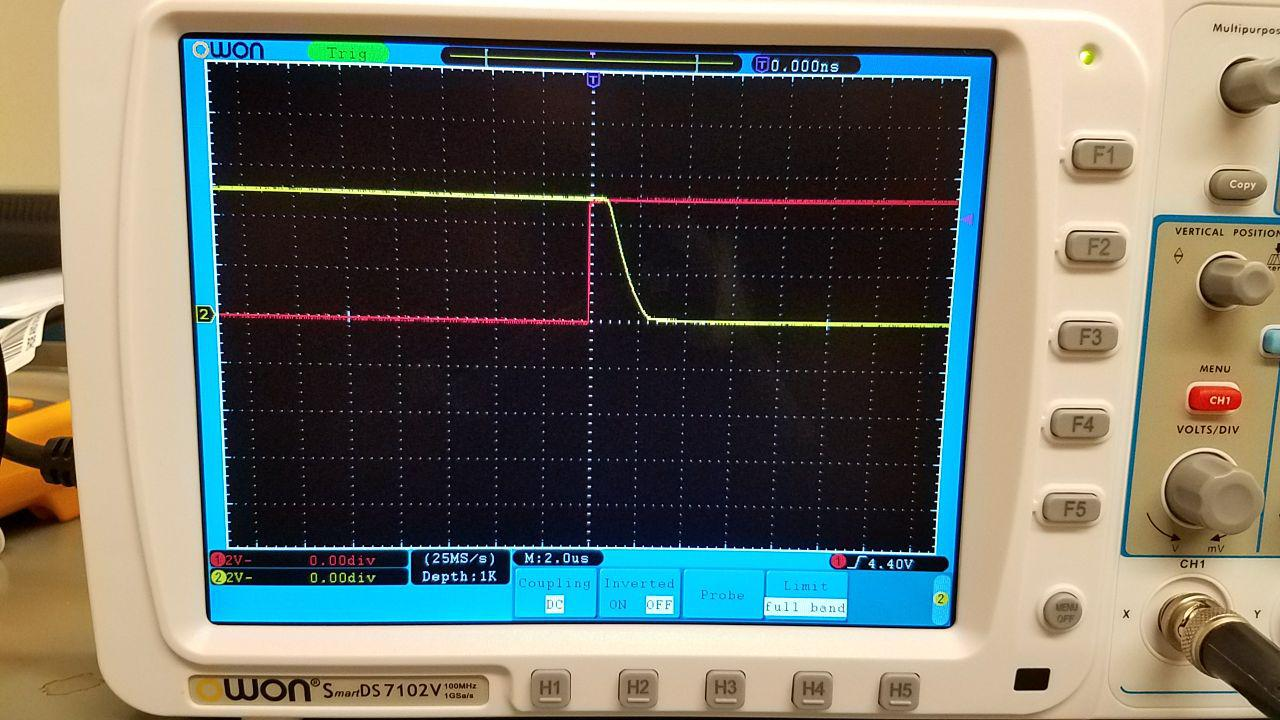
\includegraphics[width=\columnwidth]{43-NoCap.eps}
	\caption{Time delay at 100kHz from on to off.}
	\end{figure}
	
	\begin{figure}[H]
	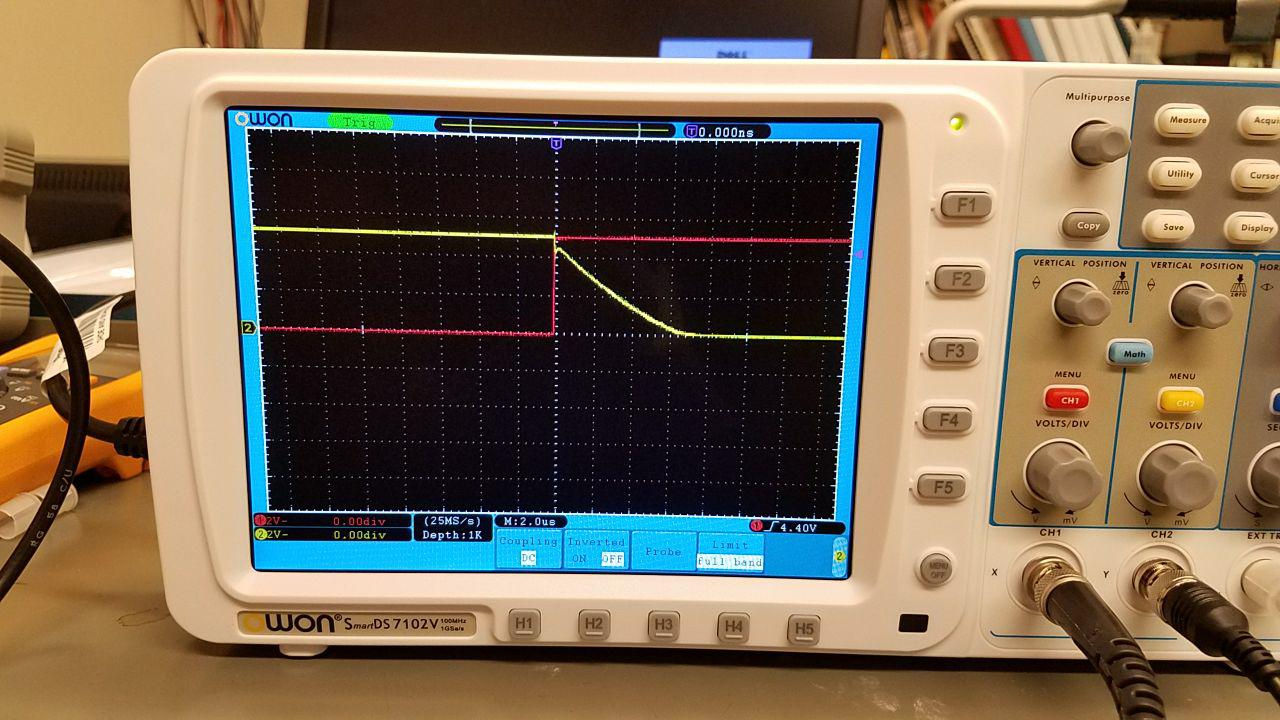
\includegraphics[width=\columnwidth]{43-WithCap.eps}
	\caption{Time delay at 100kHz from on to off.}
	\end{figure}
	
\section{Discussion}
	
	\subsection{4-1: Electromechanical Relay Switches}
	
	With the SPDT 5V electromechanical relay switch, we were able to hear an audible tick when the switch
	was changing positions. This is because there is a literal arm being moved due to our voltage coming
	into our micro relay. We found that at a low frequency, the overall voltage was incredibly low. If
	we upped the frequency to 50Hz, it got higher, and higher so for 75Hz.
	
	You can also hear when the latch when it fails, because it no longer triggers. We get an interesting
	stutter at 145Hz, and complete failure at 160Hz.
	
	Looking further and zooming in, we can see instability when each transition happens with the switch.
	This is because the switch is a physical arm (or pole) being moved back and forth between two terminals
	or throws. When it hits one of these, because of the speed at which it's doing so, you're going to get a
	bounce from the physical impact. Since the potential doesn't change, there is a restoring force that
	dampens this effect until it stabilizes again. 

	\subsection{4-2: Solid-State Switches}
	
	One thing that seems off about this circuit diagram compared to our previous one, is the requirement of
	extra input voltages. This seems like an interesting overhead cost of a solid-state relay (SSR) switch compared
	to an electromechanical relay (EMR) switch. This one doesn't make any noise, though, and thus, doesn't seem to 
	have physical moving parts like the EMR switch does. This can be a benefit, especially with how noisy the
	EMR switch was. Though there is a delay for time on and time off, if this is constant, it can be factored
	into calculations. With less moving parts as well, the failure rate seems lower than an EMR switch.
	
	\subsection{4-3: Transistor Switches}
	
	For the transistor circuit, there is a very small delay for the transition when we don't use a capacitor,
	but when we involve a capacitor, there we see an instant drop in our output voltage for a small moment, 
	before we see an exponential decay due to the capacitor's ability to store potential. Though the delay
	is no longer there, we have long transition times, were as without the capacitor, we had a delay, but
	a very short transition time.

\section{Conclusion}

From EMR, to SSR, to Transistor switches, we see that there can be common uses to each of these, depending
on granularity, overhead cost (both in cost of electricity, and cost of parts), ease of use, and longevity.
It seems that all 3 types of switches have their applications, and we demonstrate their our ability to use
them in this Laboratory, so their implementation is up to situation.

\end{document}